% D.40 反比例 y=k/x 与 y=x-2 交于 A、B
\documentclass[tikz,border=4pt]{standalone}
\usepackage{ctex}
\usepackage{amsmath}
\usetikzlibrary{calc}
\begin{document}
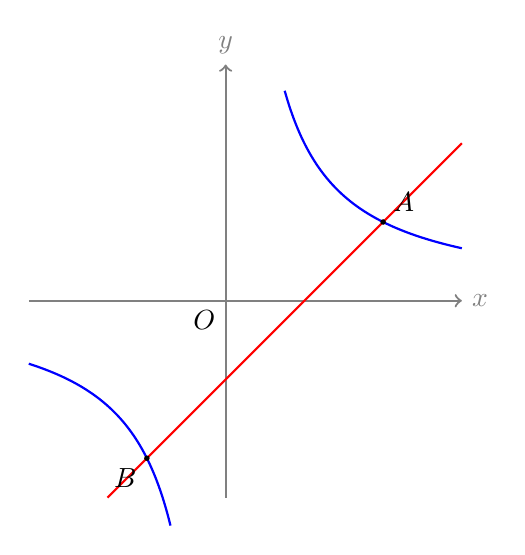
\begin{tikzpicture}[scale=0.5, thick, declare function={f(\x)=8/\x;}]
  \draw[gray, ->] (-5, 0) -- (6, 0) node[right] {$x$};
  \draw[gray, ->] (0, -5) -- (0, 6) node[above] {$y$};

  \draw[domain=1.5:6, smooth, samples=60, blue] plot (\x, {8/\x});
  \draw[domain=-5:-1.4, smooth, samples=60, blue] plot (\x, {8/\x});
  \draw[domain=-3:6, red] plot (\x, \x - 2);

  % 交点：y=k/x, y=x-2，k=8 时 x²-2x-8=0 → x=4 或 -2
  \coordinate (A) at (4, 2);
  \coordinate (B) at (-2, -4);
  \fill (A) circle (2pt); \node[above right] at (A) {$A$};
  \fill (B) circle (2pt); \node[below left]  at (B) {$B$};
  \node[below left] at (0,0) {$O$};
\end{tikzpicture}
\end{document}
